\documentclass[conference]{IEEEtran}
\IEEEoverridecommandlockouts

\usepackage[T1]{fontenc}
\usepackage{cite}
\usepackage{amsmath,amssymb,amsfonts}
\usepackage{graphicx}
\usepackage{booktabs}
\usepackage{array}
\usepackage{textcomp}
\usepackage{xcolor}
\usepackage{balance}
\usepackage{url}

\newcommand{\regret}{\rho}
\newcommand{\todo}[1]{\textcolor{red}{[#1]}}

\begin{document}

\title{Measured, Not Assumed: Benchmarking Rule-Based, Game-Theoretic and Reinforcement-Learning Response Selection for Residential IoT Defense}

\author{
\IEEEauthorblockN{Abdullah}
\IEEEauthorblockA{Dept.\ of CSE, BMSIT\&M\\
[email]}
\and
\IEEEauthorblockN{\todo{Co-author 2}}
\IEEEauthorblockA{Dept.\ of CSE, BMSIT\&M\\
\todo{email}}
\and
\IEEEauthorblockN{\todo{Co-author 3}}
\IEEEauthorblockA{Dept.\ of CSE, BMSIT\&M\\
\todo{email}}
\and
\IEEEauthorblockN{\todo{Guide}}
\IEEEauthorblockA{Dept.\ of CSE, BMSIT\&M\\
\todo{email}}
}

\maketitle

\begin{abstract}
Home IoT defenses increasingly respond to attacks automatically, but the choice of response (block, throttle, quarantine, decoy) usually comes from a hand-written playbook whose effectiveness is assumed, not measured. We build a measured-outcome benchmark for response selection in residential IoT: 693 live Mininet measurements of ten responses against 21 traffic situations (twenty attacks and normal traffic), scored by one objective that trades containment, service continuity and intelligence gain against response cost. A hand-written playbook loses 3.00 utility points on average to the best response and picks it in 4 of 21 situations. A Stackelberg game that models the attacker's reaction, built from mechanism priors alone, picks it in 20 of 21 and reaches 99.4\% of the best attainable utility. The same priors without the attacker's reaction lose 0.549, and a PPO agent trained on that attacker-blind model loses 0.577, more than ten times as much. Trained on the measurements themselves, PPO and Stackelberg are statistically indistinguishable in live paired trials ($p=0.69$): modelling the attacker removes the need to measure, it does not beat learning. A live defender recovers the correct name of all 16 single-source attacks on the lab captures it was developed on, but its rule-based detector does not transfer: on 5.5 hours of Amazon Echo traffic it would take 17--21 firewall actions per hour, and on real malware captures it never labels command-and-control as such. The evidence rests on three repetitions per cell, scripted attackers and a five-host lab; we state where each result is in-sample.
\end{abstract}

\begin{IEEEkeywords}
Internet of Things, intrusion response, Stackelberg game, reinforcement learning, benchmark, smart-home security
\end{IEEEkeywords}

%--------------------------------------------------------------------
\section{Introduction}
\label{sec:intro}
Consumer IoT devices are numerous, long-lived and rarely patched, and botnets such as Mirai showed how quickly they become attack infrastructure \cite{antonakakis2017mirai}. Most cannot run security agents, so automated defense sits at the home gateway, where it can act on the network: block an address, rate-limit a flow, quarantine a host, or redirect an attacker to a decoy.

Research has concentrated on \emph{detecting} attacks and has produced several labelled datasets \cite{garcia2020iot23,meidan2018nbaiot,koroniotis2019botiot,neto2023ciciot}. Detection alone does not protect a household: something must choose a \emph{response}, and every response has a price. Blocking a source can be useless against a spoofed flood, isolating a device stops the attack and the camera with it, and a decoy is valuable only if the attacker is still there. In practice a playbook maps an attack label to a fixed response, and game-theoretic \cite{manshaei2013game,tambe2011security,alpcan2010network} and reinforcement-learning \cite{nguyen2021deep,standen2021cyborg} response research is usually evaluated in a simulator or against the assumptions used to build the policy. We learned the cost of that first-hand: our first evaluation scored each policy by agreement with a registered ``preferred action'' for each attack, the same table the policies had been built toward, and reported 99.6\% agreement that meant nothing.

This raises a central question: can a defender choose well \emph{without} first measuring every response, and what does modelling the attacker buy? We answer it by replacing assumption with measurement. The main contributions are:
\begin{enumerate}
\item \textbf{Measured-outcome benchmark:} 693 live measurements of ten responses against twenty attacks and normal traffic (Section~\ref{sec:benchmark}). We know of no public table of this kind.
\item \textbf{Non-circular evaluation:} policies are graded against measurement, never against the data they were built from; the one variant trained on the benchmark is reported as a labelled, circular reference (Section~\ref{sec:eval}).
\item \textbf{Attacker-reaction ablation:} the same priors without the attacker's reaction have thirteen times the regret, and a PPO trained on them inherits the error (Section~\ref{sec:eval-rq2}).
\item \textbf{Live defender and naming analysis:} how an attack's name evolves as evidence accumulates, and a re-decision rule that names all 16 single-source lab attacks correctly (Sections~\ref{sec:live} and~\ref{sec:eval-rq4}).
\item \textbf{Transfer test and negative result:} the detector's thresholds, tuned on lab traffic, do not transfer to public IoT traffic (Section~\ref{sec:eval-rq5}).
\end{enumerate}

%--------------------------------------------------------------------
\section{Related Work}
\label{sec:related}
Detection datasets (N-BaIoT, Bot-IoT, IoT-23, CICIoT2023) label \emph{traffic} \cite{meidan2018nbaiot,koroniotis2019botiot,garcia2020iot23,neto2023ciciot}, and Sivanathan et al.\ characterise normal device behaviour \cite{sivanathan2019classifying}; none records what a \emph{response} does to an attack or to legitimate service. Stackelberg models underlie deployed security-resource allocation \cite{tambe2011security} and are surveyed for networks in \cite{manshaei2013game,alpcan2010network}; their payoffs are normally assumed. Deep RL for security is surveyed in \cite{nguyen2021deep}; CybORG \cite{standen2021cyborg} models enterprise networks with abstract actions, not residential IoT with concrete firewall responses. MITRE D3FEND catalogues countermeasures qualitatively \cite{kaloroumakis2021d3fend}.

Three limitations recur. First, response effectiveness is assumed or simulated, not measured against live attack traffic. Second, evaluation shares its assumptions with the policy under test, so agreement is mistaken for accuracy. Third, detectors are validated on the lab traffic that tuned them; Sommer and Paxson warn that such detectors transfer poorly to operational networks \cite{sommer2010outside}. This work addresses all three: a measured benchmark, grading that never reuses a policy's own assumptions, and a transfer test on public traffic that was not used for tuning.

%--------------------------------------------------------------------
\section{Problem Formulation}
\label{sec:problem}
Let $X$ be a set of traffic situations ($|X|=21$) and $A$ a set of responses ($|A|=10$). A detector maps traffic to a label $\hat{x}$ and a policy $\pi$ maps it to a response $\pi(\hat{x})\in A$. Applying $a$ in situation $x$ yields three measured quantities: \emph{containment} $c\in[-1,1]$ (the fraction of the un-responded attack's packets that no longer reach the protected host), \emph{service} $s\in[0,1]$ (the fraction of legitimate probe traffic that survives) and \emph{intelligence} $i\in\{0,1\}$ (verified evidence about the attacker). The realised utility is
\begin{equation}
U(x,a)=w_c\,c+w_s\,s+w_i\,i-k(a),
\label{eq:utility}
\end{equation}
with $(w_c,w_s,w_i)=(5,3,2)$ chosen by the authors and shared by every policy, and costs $k(a)$ given in Section~\ref{sec:benchmark}. For normal traffic the containment and intelligence terms are omitted, so the best utility is 3.00 (do nothing). With $\bar U(x,a)$ the mean of repeated measurements, the \emph{regret} of a policy is
\begin{equation}
\regret(\pi,x)=\max_{a\in A}\bar U(x,a)-\bar U\big(x,\pi(x)\big),
\label{eq:regret}
\end{equation}
zero exactly when the policy chooses the measured-best response. \textbf{Threat model:} an external attacker or a compromised device acts against a protected host; the defender observes traffic and applies one response at a time. Attackers are scripted; in four \emph{distributed} attacks the traffic comes from several spoofed sources, and in one experiment the attacker rotates its source after being blocked.

%--------------------------------------------------------------------
\section{The Measured-Outcome Benchmark}
\label{sec:benchmark}
\textbf{Testbed.} We use Mininet \cite{lantz2010network} with five virtual hosts, including a protected sensor, a camera as the legitimate client, and an attacker. The 20 attacks are volumetric (DoS, SYN and ICMP flood, slow loris, DNS amplification, MQTT flood), probing and credential (port scan, brute force, credential replay), payload (exploit injection, buffer-overflow probe), inside/outbound (data exfiltration, DNS tunneling, firmware tampering, rogue config beacon, C2 beaconing), and four distributed spoofed variants (DoS, SYN, ICMP, credential replay).

\textbf{Responses.} The ten responses and costs $k$ are ALLOW (0), ALERT (0.1; log only), FORENSIC\_CAPTURE (0.3; record evidence), BANDWIDTH\_CAP (0.3), BLOCK\_SOURCE (0.3; drop the source's traffic), THROTTLE (0.4; rate-limit it), RESET\_SESSIONS (0.4), DECOY (0.5; redirect it to a decoy), QUARANTINE (0.7; cut the offending host off) and ISOLATE (1.0; disconnect the protected device).

\textbf{Protocol.} For each situation we run three blocks; in each, the un-responded attack runs once to fix a baseline and each response is then applied and measured: 11 rows per block, 693 rows in all. Containment is one minus the ratio of attack packets reaching the protected host's firewall counter to the baseline, clipped to $[-1,1]$ because counts vary. Service is measured by probes from the camera to the sensor during the response. Intelligence is 1 when a decoy hit or captured evidence verifies attacker behaviour. A row is invalid only if its probe is unusable or its baseline has fewer than three packets; failed responses are kept, since dropping them would favour responses that always work. All 693 rows are valid.

\textbf{What it shows} (Fig.~\ref{fig:heat}). \emph{No response dominates:} BLOCK\_SOURCE is best in 11 situations, QUARANTINE in 7, THROTTLE in 2 and ALLOW in 1. \emph{The obvious response fails where the attack is harder:} BLOCK\_SOURCE contains 100\% of single-source attacks at cost 0.3, but about 0\% of the five inside/outbound attacks and 17--20\% of the distributed ones, whose sources are spoofed. \emph{Containment alone is not enough:} ISOLATE contains every attack yet scores 4.00 because it removes all service, and QUARANTINE contains every attack at cost 0.7 but scores $-0.70$ on normal traffic. \emph{Intelligence is rarely free:} only FORENSIC\_CAPTURE yields evidence everywhere (4.4--5.1, since it contains nothing); DECOY yields it only against the port scan.

\begin{figure*}[t]
\centering
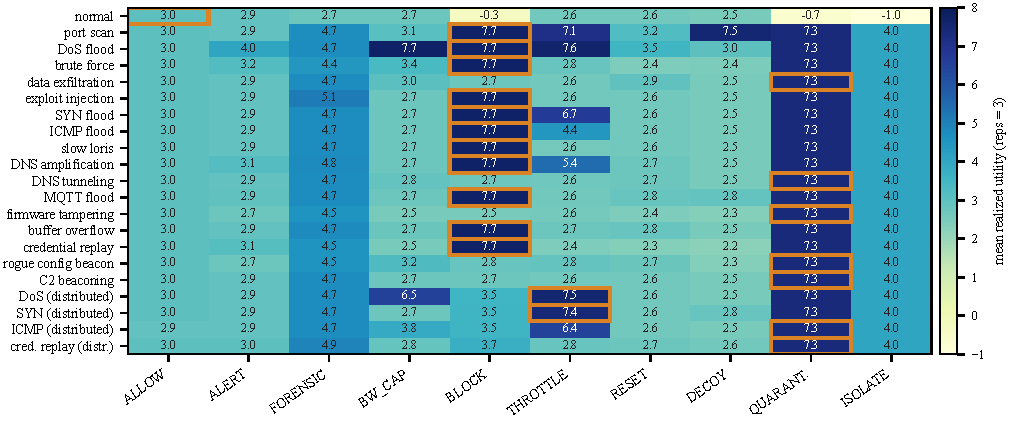
\includegraphics[width=0.88\textwidth]{figs/fig_heatmap.pdf}
\caption{The record book: mean realised utility of every response in every situation (3 repetitions). Orange outlines mark the measured-best response; ties are outlined together.}
\label{fig:heat}
\end{figure*}

%--------------------------------------------------------------------
\section{Response-Selection Policies}
\label{sec:policies}
\begin{figure*}[t]
\centering
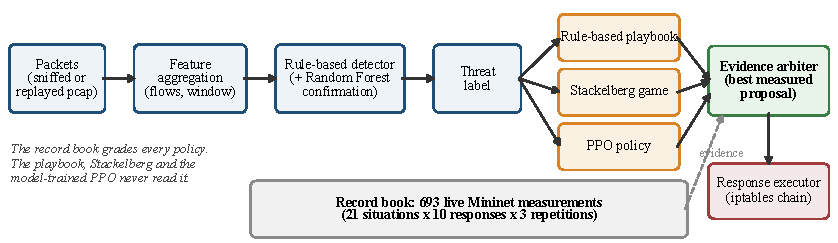
\includegraphics[width=0.74\textwidth]{figs/fig_arch.pdf}
\caption{System overview. A detector labels the traffic; three policies each propose a response; an arbiter executes the proposal with the best measured evidence. The record book grades every policy.}
\label{fig:arch}
\end{figure*}

\textbf{Rule-based playbook.} It maps each detected attack to a fixed response from general security practice (port scan $\to$ DECOY, flood $\to$ ISOLATE, brute force $\to$ BLOCK\_SOURCE) and never sees a measurement. It represents the practice we test.

\textbf{Stackelberg game from mechanism priors.} The defender (leader) commits to a response $a$; the attacker (follower) then chooses \textsc{Continue} or \textsc{Retreat}. Each attack belongs to one of nine mechanism classes. A configuration file states, for each response and class, a prior containment $e$, and for each response a prior service loss $\sigma$ and intelligence $\iota$, written from the mechanism of the response and never read from a measurement. With attacker gain $G=5$ and exposure penalty $P=2$, the attacker earns $G(1-e)-Pe$ for \textsc{Continue} and $0$ for \textsc{Retreat}, and the defender earns
\begin{align}
u_D(a,\textsc{Continue}) &= w_c e + w_s(1-\sigma) + w_i\iota - k(a),\\
u_D(a,\textsc{Retreat}) &= w_c + w_s(1-\sigma) - k(a),
\end{align}
choosing $a$ to maximise $u_D$ against the attacker's best reply. The second line matters: when the attacker is deterred there is nothing left to observe, so a response chosen for its intelligence yield earns none of it. An optional follower action, \textsc{Rotate-Source}, models an attacker who attacks from a fresh address and nullifies responses keyed on the old one. The priors were written by authors who knew the lab, so we do \emph{not} claim Stackelberg is evaluated blind; Section~\ref{sec:eval-rq2} isolates what its structure contributes.

\textbf{PPO as a contextual bandit.} Decisions are independent, so we train PPO \cite{schulman2017ppo,raffin2021sb3} with $\gamma=0$: a 31-dimensional observation (six numeric detector features, a 21-way attack label, a four-way intention), a $64\times64$ MLP and 120{,}000 steps. The label seen is wrong 15\% of the time, and the reward is the realised utility of the response in the \emph{true} situation divided by ten. \textbf{PPO-M} (model-trained) computes utility from the same priors, without the attacker's reaction, and sees no measurement. \textbf{PPO-R} (record-book-trained) samples measured rewards; because the benchmark is also the answer key, its score on known attacks is circular and is shown only as a reference.

\textbf{Evidence arbiter.} The arbiter looks up each proposal's measured outcomes and executes the one with the highest mean minus one standard deviation, breaking ties in the order Stackelberg, PPO, playbook. It ignores the detector's confidence, which is not comparable across policies.

%--------------------------------------------------------------------
\section{The Live Defender and its Detector}
\label{sec:live}
\textbf{Detection.} Packets are aggregated into thirteen behavioural features (protocol, duration, packet count and rate, bytes, mean size, distinct ports, SYN/ACK/UDP/ICMP counts, inter-arrival variation). One small rule set per attack, with non-overlapping signatures, runs on every capture; a Random Forest \cite{breiman2001random} (64 trees, 260 flows) confirms port scans. Thresholds were calibrated on lab traffic.

\textbf{Pipeline.} The defender sniffs a named interface, keeps a rolling window, runs the detectors every second and acts on a source only after two consecutive flagged checks. Responses are real firewall rules in a dedicated iptables chain hooked only to that interface; the host, the gateway and any client that completes real requests are never blocked; blocks expire after 60~s. Five responses can be applied on this device (ALLOW, ALERT, FORENSIC\_CAPTURE, BLOCK\_SOURCE, THROTTLE); other proposals are set aside and reported.

\textbf{Naming an attack takes evidence.} The opening packets of one attack resemble another, so a defender acting at its first confirmation may act on the wrong name. We add a longer window over traffic in \emph{both} directions (the rules were tuned on captures containing both, and inside attacks show only as outbound traffic) and \emph{re-decision}: after acting, the defender keeps reading the source and, if the name changes to one it has not held before and stays changed for two checks, decides again, applying the new response only if it differs (at most twice per source; it never returns to an abandoned name, since once the attack leaves the window the label drifts and that drift is not new information).

%--------------------------------------------------------------------
\section{Evaluation}
\label{sec:eval}
\textbf{Questions.} RQ1: how much does a playbook lose? RQ2: does modelling the attacker's reaction matter? RQ3: what does learning add? RQ4: can the live defender name every attack? RQ5: does the detector transfer to real IoT traffic?

\textbf{Setup.} Policies are graded by regret (Eq.~\ref{eq:regret}) against the benchmark (``table-graded''), or by applying their choices live and measuring afresh (``live paired trials'': 8 trials in each of the 21 situations, 168 in all, one shared detector of 97.6\% accuracy, so differences come from the policies). Everything ran in Python~3.12 on a two-vCPU, 3~GB virtual machine without a GPU, using Mininet, Scapy and iptables; PPO used Stable-Baselines3 on CPU. PPO-M used seeds 1, 7 and 13 (about 7 minutes each); PPO-R used seed 7, with ten seeds for robustness.

\textbf{Statistical treatment.} Intervals are 95\% percentile-bootstrap intervals over trials \cite{efron1993bootstrap} or Wilson intervals for proportions \cite{wilson1927probable}; paired comparisons use the Wilcoxon signed-rank test \cite{wilcoxon1945individual} with Holm adjustment \cite{holm1979simple} over the three comparisons among the playbook, Stackelberg and PPO, which leaves every conclusion below unchanged. Trials share one testbed and are not independent of its drift, and the benchmark has only three repetitions per cell, so the intervals should be read as lower bounds on the true uncertainty. Table-graded regret uses the same repetitions that define the best response, which biases regret slightly upward for any policy that does not pick the selected maximum; the live trials are fresh measurements.

\subsection{RQ1: a playbook loses about three points}
\label{sec:eval-rq1}
Table~\ref{tab:main} gives table-graded results. The playbook's mean utility is 4.33 against 7.32 for the lookup of the best row (mean regret 3.00), and it picks the measured-best response in 4 of 21 situations. In live trials (Table~\ref{tab:live}) it contains 53.9\% of attack traffic with 30.4\% service loss, against 98.3\% and 1.7\% for Stackelberg. The errors are structural: exploit injection $\to$ DECOY scores 2.50 where BLOCK\_SOURCE scores 7.70, and DoS flood $\to$ ISOLATE scores 4.00 because it removes the service it protects.

\begin{table}[t]
\caption{Table-graded results over the 21 situations. ``Best'' counts situations where the policy chooses the measured-best response. PPO-M is the mean of three seeds. Best non-circular result in bold.}
\label{tab:main}
\centering
\scriptsize
\setlength{\tabcolsep}{4pt}
\begin{tabular}{@{}lcccc@{}}
\toprule
Policy & Utility & Regret & Worst & Best \\
\midrule
Lookup of the best row (ceiling) & 7.322 & 0.000 & 0.00 & 21 \\
\midrule
Rule-based playbook & 4.326 & 2.996 & 5.20 & 4 \\
Fixed QUARANTINE & 6.919 & 0.403 & 3.70 & 7 \\
Priors, no attacker (argmax) & 6.773 & 0.549 & 5.25 & 17 \\
PPO-M (model-trained) & 6.745 & 0.577 & 5.25 & 15.7 \\
Stackelberg (priors only) & \textbf{7.280} & \textbf{0.042} & \textbf{0.88} & \textbf{20} \\
\midrule
PPO-R (record-book-trained)$^{\dagger}$ & 7.305 & 0.017 & 0.24 & 19 \\
\bottomrule
\multicolumn{5}{@{}p{0.95\columnwidth}@{}}{\scriptsize $^{\dagger}$Trained on the data it is graded on: a circular reference, not independent evidence.}
\end{tabular}
\end{table}

\subsection{RQ2: the attacker's reaction is the ingredient that matters}
\label{sec:eval-rq2}
Stackelberg and the ``priors, no attacker'' row use \emph{identical} numbers and differ only in whether the attacker's reaction is modelled: regret 0.042 against 0.549. The authors' knowledge of the lab affects both rows equally and cancels, so this is the cleanest evidence that the structure of the model, not the tuning of its numbers, carries the result. PPO-M, trained on the attacker-blind model, inherits its errors: it reproduces the model's own best response in 84\% of situations and chooses DECOY for exploit injection and the buffer-overflow probe (regret 5.20 and 5.25).

The mechanism is visible in the payoffs. For exploit injection the attacker-blind model values DECOY at 7.95 and BLOCK\_SOURCE at 7.20 because DECOY promises intelligence. With the attacker's reaction, continuing against either is unprofitable ($-0.6$ and $-1.3$), so the attacker retreats, DECOY's intelligence is never earned, and the game values DECOY at 7.35 and BLOCK\_SOURCE at 7.70. Measurement agrees: 2.50 and 7.70. Stackelberg's only miss is the distributed ICMP flood (regret 0.88): its prior favours THROTTLE, which drops the legitimate probe (33\% service loss).

\subsection{RQ3: learning helps where measurements exist}
\label{sec:eval-rq3}
\textbf{With measurements, PPO ties Stackelberg.} Table~\ref{tab:live} gives the live paired trials. Stackelberg and PPO-R differ by $+0.027$ [0.00, 0.06] ($p=0.69$; 24 of 168 trials differ): the interval contains zero and the comparison is not significant. The arbiter, which equals the best of the three proposals in every trial, is marginally higher (+0.044, $p=0.008$, but only 8 trials differ). Across ten seeds PPO-R's mean regret is 0.017 (worst 0.022). The claim ``Stackelberg is best'' is therefore not supported; the supported claim is that, with no measurement, it is within 0.6\% of the ceiling.

\begin{table}[t]
\caption{Live paired trials (168 trials; each response applied and measured). $\Delta$ is the paired difference from Stackelberg with its 95\% bootstrap interval; $p$ is the two-sided Wilcoxon signed-rank test.}
\label{tab:live}
\centering
\scriptsize
\setlength{\tabcolsep}{2pt}
\begin{tabular}{@{}lccc@{}}
\toprule
Policy & Utility [95\% CI] & $\Delta$ [95\% CI] & $p$ \\
\midrule
Rule-based & 4.272 [4.00, 4.56] & $-2.954$ [$-3.26$, $-2.64$] & $1.9\times10^{-22}$ \\
Stackelberg & 7.226 [7.04, 7.38] & --- & --- \\
PPO-R$^{\dagger}$ & 7.254 [7.08, 7.40] & $+0.027$ [0.00, $+0.06$] & 0.69 \\
Arbiter & \textbf{7.271} [7.09, 7.42] & $+0.044$ [$+0.016$, $+0.081$] & 0.008 \\
Block all & 3.940 [3.90, 3.97] & $-3.286$ [$-3.41$, $-3.14$] & $5.1\times10^{-29}$ \\
Allow all & 3.000 [3.00, 3.00] & $-4.226$ [$-4.38$, $-4.04$] & $5.1\times10^{-29}$ \\
\bottomrule
\end{tabular}
\end{table}

\textbf{Unseen attacks.} Holding each attack out of PPO-R's training, its regret on the held-out attack is 1.61 [0.85, 2.47] (best in 3 of 20) against 0.04 [0.00, 0.13] (19 of 20) for Stackelberg and the arbiter. PPO cannot generalise because attack identity is an input; Stackelberg does not learn, so this shows only that a mechanism-class prior transfers to an unseen attack where a learned table does not.

\textbf{Noisy detector and reactive attacker} (simulated labels and a scripted attacker; PPO trained on the benchmark, so indicative only). At a realistic 90\% benign mix a noise-aware PPO beats Stackelberg by 0.29--0.56 regret when 20--30\% of labels are wrong (0.36 against 0.89 at 30\% uniform error) and costs 0.21 when the detector is accurate. When the attacker switches source after a source-keyed response, BLOCK\_SOURCE contains 0\% instead of 100\%; deployed Stackelberg and PPO carry regret 2.17, a rotation-aware Stackelberg 0.56 (1.19 against a non-reactive attacker), and a PPO trained on the adaptive table 0.07 in sample.

\subsection{RQ4: naming every attack correctly}
\label{sec:eval-rq4}
We replayed 5 saved captures of each of the 16 single-source attacks through the complete defender (detection, policy pipeline, response executor, recording firewall). With the original configuration (last 5~s of inbound traffic, one decision per source) the defender ends on the correct name for 7 of 16 attacks; with a 60~s window over both directions and re-decision it does so for all 16, with no false alarms on normal captures (Fig.~\ref{fig:labels}). \emph{This is a development-set result:} the thresholds were tuned on these attacks and the re-decision rule was designed after inspecting these captures, so it is not a held-out estimate. The right name arrives after 1--3~s for floods, scans and brute force, 3--10~s for DNS amplification, exfiltration, rogue beacon, firmware tampering and DNS tunneling, and 17--32~s for credential replay, C2 beaconing, slow loris, the buffer-overflow attack and the MQTT flood; the original configuration never acts on exfiltration, credential replay, firmware tampering or the MQTT flood.

\begin{figure}[t]
\centering
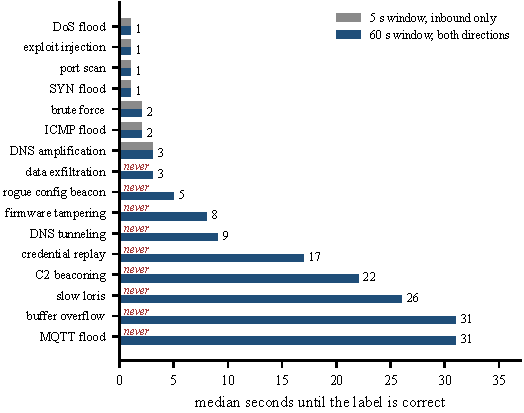
\includegraphics[width=0.9\columnwidth]{figs/fig_labels.pdf}
\caption{Median seconds until the defender's label is correct. ``Never'': the original configuration does not reach the right name.}
\label{fig:labels}
\end{figure}

Names are right but responses are not always best: for exfiltration, C2, DNS tunneling and firmware tampering the final decision still has regret about 1.8 against the best response the device can apply, because the policies propose responses (QUARANTINE, ISOLATE) it cannot apply and the arbiter falls back to ALERT, whereas FORENSIC\_CAPTURE would score 4.70. This limits arbitration among proposals, not detection. The four distributed attacks have no saved captures (live-trial detector accuracy 98\% [94, 99\%]). In one qualitative physical run (laptop attacker, phone client, defender in a VM on a bridged adapter) a real \texttt{nmap} scan was detected and blocked while the phone's page stayed reachable.

\subsection{RQ5: the detector does not transfer}
\label{sec:eval-rq5}
\textbf{Lab accuracy is in-sample.} Saved lab captures are classified correctly 100\% of the time [98, 100\%] (279 captures), live trials 98\%, and a Random Forest 99\% in five-fold cross-validation by run. These must not be quoted as general performance: thresholds were hand-placed against those attacks, and moving each feature of an attack's signature by up to $\pm30$\% leaves the correct label in only 29--100\% of cases.

\textbf{Real traffic.} We replayed IoT-23 \cite{garcia2020iot23,paxson1999bro} with nothing tuned on it: 5.5~h and 396{,}648 packets of one benign Amazon Echo, and six malware captures (chosen for size, two truncated to their first 30~min). Both configurations are scored with the same 60~s matching window, so the comparison is like for like. \emph{Benign traffic is mis-handled:} the Echo is flagged in 159 (original configuration) and 594 (60~s window, both directions) seconds per hour, and the defender would take 95 and 116 firewall actions in 5.5~h (17 and 21 per hour, counting a 60~s block as one action), read as exploit injection, flood and brute force. \emph{Scanning is recognised:} on the scanning malware (3-1) every alarm falls while a malicious connection is open, and 28\% of its connections (9\% originally) are followed by an alarm with a plausible name (scan or brute force). \emph{Command and control is noticed, not named:} the longer window raises the share of connections followed by an alarm from 73\% to 98\% (Mirai) and from 50\% to 81\% and 71\% (Torii), but none of the 314 command-and-control connections receives a beacon-like name in either configuration; they are called brute force, credential replay or MQTT flood. The quiet capture 8-1 is not noticed at all (0 of 8{,}222 connections). \emph{A noisy device swamps real alarms:} in the trojan capture (42-1) all six connections are followed by an alarm, but 99\% of alarms occur while nothing malicious is open, so ``noticed'' is uninformative there. Table~\ref{tab:public} gives the details.


\begin{table}[t]
\caption{IoT-23 malware captures; every cell is original configuration / 60~s window, both directions, scored with one 60~s matching window (3-1 and 34-1: first 30~min). Noticed: malicious connections followed by an alarm; precision: alarms raised while a malicious connection was open; named: connections followed by an alarm whose name fits IoT-23's label (our judgement); actions: firewall actions with a 60~s block.}
\label{tab:public}
\centering
\scriptsize
\setlength{\tabcolsep}{2.5pt}
\begin{tabular}{@{}llrcccc@{}}
\toprule
Capture & Kind & Conn. & Noticed (\%) & Prec.\ (\%) & Named (\%) & Actions \\
\midrule
3-1 & scan + attacks & 1635 & 30/43 & 100/100 & 9/28 & 2/6 \\
34-1 & Mirai C\&C & 284 & 73/98 & 83/93 & 0/0 & 14/15 \\
20-1 & Torii C\&C & 16 & 50/81 & 100/84 & 0/0 & 1/34 \\
21-1 & Torii C\&C & 14 & 50/71 & 100/98 & 0/0 & 3/60 \\
8-1 & quiet C\&C & 8222 & 0/0 & --- & 0/0 & 0/0 \\
42-1 & trojan download & 6 & 100/100 & 4/1 & 33/0 & 82/134 \\
\bottomrule
\end{tabular}
\end{table}

\textbf{The cost of the longer window.} It finds more, and it acts far more: on the two Torii captures firewall actions rise from 1 to 34 and from 3 to 60, and on the trojan capture from 82 to 134 (Table~\ref{tab:public}). Replaying the phone traffic from our demonstration (111~s, one request every two seconds), the 60~s window flags 110 of 111 checks as brute force against 3 for the original setting: requests that are harmless over 5~s accumulate into the pattern of a login attack over 60~s. The phone is not blocked because the defender trusts a client after two real requests, but any other regularly polling device would be; we keep the original configuration for live use until a per-device baseline replaces fixed thresholds.

\textbf{Cost and scalability.} Decisions take 0.05~ms (playbook), 0.46~ms (Stackelberg) and 1.14~ms (PPO). The real cost is measurement: a new attack adds 33 rows and a new response 63, and the 168-trial live harness took 2.0~h.

%--------------------------------------------------------------------
\section{Discussion}
\label{sec:discussion}
\textbf{What the results show.} Playbooks lose heavily when measured. Modelling the attacker's reaction, with no measurement, recovers almost all the attainable utility. A learned policy needs measurements: trained on an attacker-blind model it repeats the model's mistakes, trained on measurements it ties the game. The results do \emph{not} show that ``Stackelberg is best for home IoT'': live trials tie, a noise-aware PPO is better under a noisy detector, and an adaptive PPO is better against a reactive attacker (in sample). Reporting the 100\% lab detection accuracy without the 29\% margin under perturbation, the 17--21 firewall actions per hour on a benign device and the missing C\&C labels would misrepresent the detector. The lookup of the best row is the ceiling only for situations already measured, in the lab, with a correct label; a home defender has no such table, so the policies are what it uses and the benchmark is how they are graded.

\textbf{Limitations.} The most consequential are statistical and structural: three repetitions per cell, five virtual hosts, scripted attackers, and a baseline of only 4--20 packets for several attacks, so differences of a few hundredths of regret should not be over-read. The priors were written by authors who knew the lab and were committed together with the measured evaluation, after a preliminary measurement run had been made, so we cannot show they were written blind (the ablation of Section~\ref{sec:eval-rq2} is unaffected because both rows share them). PPO-R trains on the data it is graded on, so the headline rests on Stackelberg, PPO-M and live trials; the noise and reactive-attacker experiments use benchmark-trained PPO and are indicative only. The naming result is a development-set result (Section~\ref{sec:eval-rq4}). The IoT-23 captures were chosen for size, the label mapping is our judgement, only one benign device was replayed, and the physical validation is one qualitative run; no result was re-measured on physical IoT hardware. All attack traffic was generated in an isolated virtual network or against the authors' own machines, and IoT-23 was only parsed.

\textbf{Future work.} Per-device behavioural baselines to cut false alarms; an arbiter that considers every response the device can apply; re-measurement on physical devices with more repetitions and an independently written prior; online learning from deployed outcomes.

%--------------------------------------------------------------------
\section{Conclusion}
\label{sec:conclusion}
Key findings: (1) a hand-written playbook loses 3.00 utility points to the measured-best response and picks it in 4 of 21 situations; (2) a Stackelberg model of the attacker's reaction, built from priors alone, reaches 99.4\% of the best attainable and picks the best response in 20 of 21; (3) the same priors without the attacker lose thirteen times as much, and a PPO trained on them inherits the loss; (4) trained on measurements, PPO and Stackelberg are statistically indistinguishable in live trials ($p=0.69$); (5) the live defender names every single-source lab attack within 1--32 seconds (a development-set result); (6) its lab-tuned detector does not transfer: 17--21 firewall actions per hour on a benign device and no beacon label on real C\&C traffic. The benchmark and harness let others add networks, devices and attacks.

\section*{Acknowledgment}
During the preparation of this manuscript, the author(s) used Claude (Anthropic) to draft and edit the text, to write and run evaluation and analysis code, and to generate figures and tables. All AI-assisted output was reviewed and, where necessary, edited by the author(s), who take full responsibility for the final content of the manuscript. \todo{Guide and funding acknowledgements; authors confirm the statement above.}

\section*{Availability}
\todo{Repository URL and data licence. IoT-23 is distributed by the Stratosphere Laboratory and was used unmodified.}

\balance
\bibliographystyle{IEEEtran}
\bibliography{refs}

\end{document}
